\documentclass[a4paper,10pt]{article}
\usepackage[utf8]{inputenc}
\usepackage{tikz}
\usepackage{amsmath}
\usepackage{fullpage}

%opening
\title{Attaque du protocole de l'équipe A Team}
\author{par l'Equipe Stone Jaws}
\date{12 octobre 2018}

\begin{document}

\maketitle

\section{Le protocole}

Considérons 3 rôles $i$, $r$, et $m$ (que l'on appellera respectivement initiateur, récepteur, et serveur). La sémantique (en utilisant les notations de \cite{cas}) de ce protocole est alors donnée par :
\begin{eqnarray*}
	TdSD(i) & = & \{ (i,r,m, K, K_{im}), \\
		& & \texttt{send}_1(i,m, \langle i, \textrm{senc}(r,K_{im})\rangle ),\\
		& & \texttt{recv}_2(m,i,\textrm{senc}(\langle r, K_{ir} \rangle,K_{im})),\\
		& & \texttt{send}_4(i,r,\textrm{senc}(K, K_{ir})),\\
		& & \texttt{recv}_5(r,i,\textrm{senc}(\langle N_b, h(K) \rangle, K_{ir})),\\
		& & \texttt{send}_6(r,i,\textrm{senc}(N_b, K_{ir}))\}
\end{eqnarray*}
\begin{eqnarray*}
	TdSD(r) & = & \{ (i,r,m, K_{rm}, N_b), \\
		& & \texttt{send}_3(m,r,\textrm{senc}(\langle i, K_{ir} \rangle,K_{rm}) ),\\
		& & \texttt{recv}_4(i,r,\textrm{senc}(K, K_{ir})),\\
		& & \texttt{send}_5(r,i,\textrm{senc}(\langle N_b, h(K) \rangle, K_{ir})),\\
		& & \texttt{recv}_6(r,i,\textrm{senc}(N_b, K_{ir}))\}
\end{eqnarray*}
\begin{eqnarray*}
	TdSD(m) & = & \{ (i,r,m, K_{rm}, K_{im}, K_{ir}), \\
		& & \texttt{recv}_1(i,m, \langle i, \textrm{senc}(r,K_{im})\rangle ),\\
		& & \texttt{send}_2(m,i,\textrm{senc}(\langle r, K_{ir} \rangle,K_{im}) ),\\
		& & \texttt{send}_3(m,r,\textrm{senc}(\langle i, K_{ir} \rangle,K_{rm}) )\}
\end{eqnarray*}


\begin{center}

\begin{figure}
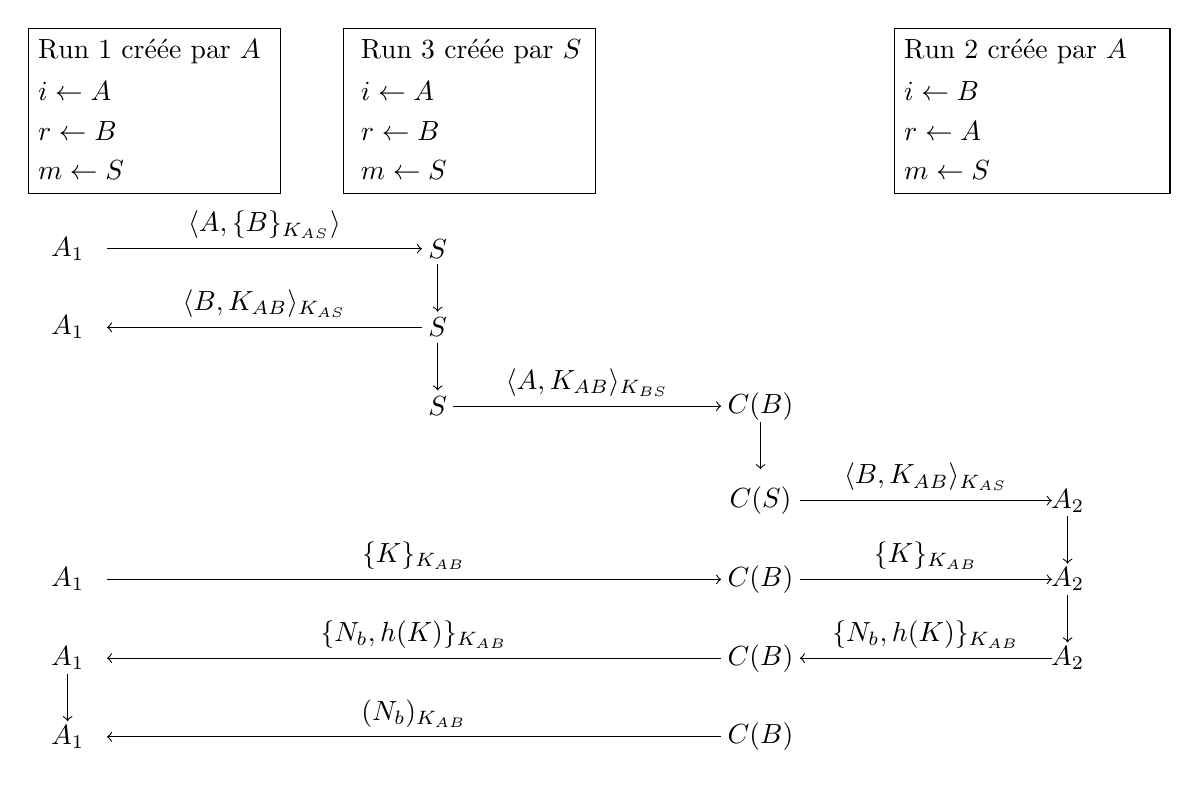
\begin{tikzpicture}
  \draw(-7,8.8) rectangle (-3.8,6.7);
	\draw (-7,8.5) node[right]{Run 1 créée par $A$};
	\draw (-7,8) node[right]{$i \leftarrow A$};
	\draw (-7,7.5) node[right]{$r \leftarrow B$};
	\draw (-7,7) node[right]{$m \leftarrow S$};

  \draw(-3,8.8) rectangle (0.2,6.7);
	\draw (-2.9,8.5) node[right]{Run 3 créée par $S$};
	\draw (-2.9,8) node[right]{$i \leftarrow A$};
	\draw (-2.9,7.5) node[right]{$r \leftarrow B$};
	\draw (-2.9,7) node[right]{$m \leftarrow S$};

	\draw(4,8.8) rectangle (7.5,6.7);
	\draw (4,8.5) node[right]{Run 2 créée par $A$};
	\draw (4,8) node[right]{$i \leftarrow B$};
	\draw (4,7.5) node[right]{$r \leftarrow A$};
	\draw (4,7) node[right]{$m \leftarrow S$};

	\draw (-6.5,6) node{$A_1$} ;
	\draw[->]  (-6,6) -- node[above]{$\langle A, \{B\}_{K_{AS}} \rangle$} (-2,6) ;
	\draw (-1.8,6) node{$S$} ;
	\draw[->]  (-1.8,5.8) -- (-1.8,5.2) ;
	\draw (-1.8,5) node{$S$} ;
	\draw[<-]  (-6,5) -- node[above]{$\langle B, K_{AB}\rangle_{K_{AS}}$} (-2,5) ;
	\draw (-6.5,5) node{$A_1$} ;
	\draw[->]  (-1.8,4.8) -- (-1.8,4.2) ;
	\draw (-1.8,4) node{$S$} ;
	\draw[->]  (-1.6,4) -- node[above]{$\langle A, K_{AB}\rangle_{K_{BS}}$} (1.8,4) ;
	\draw (2.3,4) node{$C(B)$} ;
	\draw[->]  (2.3,3.8) -- (2.3,3.2) ;
	\draw (2.3,2.8) node{$C(S)$} ;
	\draw[->]  (2.8,2.8) -- node[above]{$\langle B, K_{AB}\rangle_{K_{AS}}$} (6,2.8) ;
	\draw (6.2,2.8) node{$A_2$} ;
	\draw[->]  (6.2,2.6) -- (6.2,2) ;

	\draw (-6.5,1.8) node{$A_1$} ;
	\draw[->]  (-6,1.8) -- node[above]{$\{K\}_{K_{AB}}$} (1.8,1.8) ;
	\draw (2.3,1.8) node{$C(B)$} ;
	\draw[->]  (2.8,1.8) -- node[above]{$\{K\}_{K_{AB}}$} (6,1.8) ;
	\draw (6.2,1.8) node{$A_2$} ;

	\draw[->]  (6.2,1.6) -- (6.2,1) ;

	\draw (-6.5,0.8) node{$A_1$} ;
	\draw[<-]  (-6,0.8) -- node[above]{$\{N_b, h(K)\}_{K_{AB}}$} (1.8,0.8) ;
	\draw (2.3,0.8) node{$C(B)$} ;
	\draw[<-]  (2.8,0.8) -- node[above]{$\{N_b, h(K)\}_{K_{AB}}$} (6,0.8) ;
	\draw (6.2,0.8) node{$A_2$} ;

	\draw[->]  (-6.5,0.6) -- (-6.5,0) ;

	\draw (-6.5,-0.2) node{$A_1$} ;
	\draw[<-]  (-6,-0.2) -- node[above]{$(N_b)_{K_{AB}}$} (1.8,-0.2) ;
	\draw (2.3,-0.2) node{$C(B)$} ;
\end{tikzpicture}
\caption{Attaque du protocole A Team}
\label{fig1}
\end{figure}
\end{center}

\section{Attaque sur le protocole}
L'attaque est représentée sur la Figure \ref{fig1} et fonctionne comme suit : Alice ($A$) exécute le protocole une fois (dans la Run $1$) en tant qu'initiateur et veut s'adresser à Bob ($B$), et une autre fois (dans la Run $2$) en tant que récepteur avec $B$ dans le rôle d'initiateur. On notera $A_1$ et $A_2$ pour distinguer l'agent $A$ en tant qu'acteur des Runs $1$ et $2$.\\
\begin{enumerate}
\item $A_1$ envoie son premier message à $S$ sans encombre.
\item $S$ va répondre par deux messages, l'un pour $A$, l'autre pour $B$. Celui pour $B$ est bloqué par l'attaquant. Celui pour $A_1$, $\langle B, K_{AB} \rangle_{K_{AS}}$ est copié.
\item L'attaquant va renvoyé ce message à $A_2$ dans sa run où $A$ est récepteur. $A$ croit donc recevoir une demande de contact de $B$.
\item. Pour les trois messages suivant, l'attaquant se fait passer pour $B$ récepteur au yeux de $A_1$ et se fait passer pour $B$ initiateur aux yeux de $A_2$. Il ne fait que passer les messages de $A_1$ à $A_2$ et vice-versa.
\end{enumerate}
À la fin, $A$ pense donc avoir communiqué avec $B$ dans ses deux runs, alors que $B$ n'est jamais intervenu.

On remarque alors que deux des propriétés exigées ne sont pas vérifiées :
\begin{itemize}
\item Dans cet exemple, l'initiateur $A$ de la Run $1$ envoie un message à un récepteur $B$ et termine le protocole alors que le récepteur n'a pas reçu le message.
\item De plus, le récepteur $A$ de la Run $2$ croit recevoir une donnée d'un initiateur $B$ qui ne l'a en fait jamais envoyée.
\end{itemize}

\bibliographystyle{plain}
\bibliography{ref.bib}

\end{document}
